\documentclass[11pt]{article}

% Change "review" to "final" to generate the final (sometimes called camera-ready) version.
% Change to "preprint" to generate a non-anonymous version with page numbers.
\usepackage[preprint]{acl}

% Standard package includes
\usepackage{times}
\usepackage{latexsym}

% For proper rendering and hyphenation of words containing Latin characters (including in bib files)
\usepackage[T1]{fontenc}
% This assumes your files are encoded as UTF8
\usepackage[utf8]{inputenc}
% Improves the layout of the manuscript
\usepackage{microtype}
% Nicer typewriter font (optional; skipped if the package is not installed)
\IfFileExists{inconsolata.sty}{\usepackage{inconsolata}}{}
% For including images
\usepackage{graphicx}
% Math
\usepackage{amsmath}
\usepackage{amssymb}
\usepackage{booktabs}

\title{Local Convolutions of Token Embeddings Improve Character-Level\\
Discrete Diffusion Language Models}

\author{Arseni Ivanov \\
  Department of Computer Science \\
  Lund University \\
  \texttt{arseni.ivanov@cs.lth.se} \\}

\begin{document}
\maketitle

\begin{abstract}
Discrete diffusion language models generate text by iteratively denoising a
fully corrupted sequence in parallel, avoiding the sequential bottleneck of
autoregressive decoding. We study a compact character-level discrete diffusion
model (under 6.5M parameters) built on a DiT-style transformer and trained on
the Tiny Shakespeare corpus under a fixed two-epoch budget on a single 16~GB
GPU. Using roughly 105 controlled experiments, we study architectural and optimization choices in this constrained regime. Our main architectural result is that a small stack of depthwise convolutions on the token embeddings provides a useful local inductive bias at negligible cost, improving both validation loss and qualitative output. Established optimization techniques, particularly exponential weight averaging, provide gains of comparable magnitude. We therefore emphasize the convolution as a cost-effective and less explored architectural intervention rather than as the dominant source of overall improvement. We also report negative results for several larger architectural techniques and a forward-pass kernel optimization reaching a 1.81× speedup.
\end{abstract}

\section{Introduction}

Autoregressive language models generate text one token at a time, which imposes
three structural costs: generation is inherently $\mathcal{O}(N)$ in sequence
length; the causal factorization makes it impossible to revise or inpaint
earlier tokens without regenerating everything that follows; and decoding
becomes memory-bound as the key--value cache grows with context length.
Discrete diffusion language models
\citep{austin2021d3pm,lou2024sedd,sahoo2024mdlm} offer an alternative. Starting
from a fully corrupted sequence, the model iteratively denoises all positions in
parallel, which enables bidirectional context, inpainting, and a compute/quality
trade-off through the number of denoising steps. Recent work has scaled this
paradigm to billions of parameters \citep{nie2025llada,arriola2025block}, but
the inductive biases that make small such models train well remain understudied.

This paper studies a small character-level discrete diffusion model under fixed
hardware and training constraints. We chose discrete diffusion as the research
direction because parallel denoising removes the strict token-by-token dependency
of autoregressive decoding, offering a route toward greater generation throughput
as decoding becomes increasingly memory-bound. We use a nanoGPT
\citep{karpathy2022nanogpt} backbone adapted into a diffusion transformer (DiT)
\citep{peebles2023dit} with noise-conditioned adaptive layer normalization
(adaLN), and evaluate every configuration using the same standardized two-epoch
benchmark.

The research direction, experimental constraints, model family, and overall
experimental framing were chosen by the author. The search then explored both
established ideas from the transformer and optimization literature including
RoPE, ALiBi, QK normalization, learning-rate scheduling, and weight
averaging as well as architectural variants proposed during the autonomous loop.
The agent proposed and implemented individual experiments, ran the standardized
benchmark, and retained changes that improved validation loss. The embedding
convolution emerged from this process as an especially interesting architectural
result: its benefit is consistent with the strong short-range structure of
character-level text, where a cheap local operator can complement the global
mixing of attention during parallel denoising. Roughly 105 experiments were
logged; Section~\ref{sec:conv} discusses this result and
Section~\ref{sec:ablation} the broader ablation.

\section{Model and Training Setup}
\label{sec:method}

We use an absorbing-state (masking) forward process in the style of MDLM
\citep{sahoo2024mdlm}. A clean sequence $x_0$ is corrupted at a continuous time
$t\in[0,1]$ under a cosine noise schedule, so the probability that a token is
masked is $\bar\sigma_t = 1-\cos(t\pi/2)$, rising from about $0$ at $t{=}0$ to
about $1$ at $t{=}1$. The model $s_\theta(x_t,\bar\sigma_t)$ is trained to
recover $x_0$. We try two losses during the study: a time-conditioned masked
cross-entropy on the corrupted positions, and the score-entropy objective\cite{lou2024sedd}, in
which the rate-of-noise term $\sigma_t$ weights the per-position loss,
We find that for our experimental setup, the score-entropy objective underperforms
the simple time-conditioned cross-entropy.

The backbone is a pre-norm transformer with per-block adaLN modulation that
derives shift, scale, and gate vectors from a sinusoidal embedding of the noise
level \citep{peebles2023dit}. Onto this backbone we layered the components found
during the search (Section~\ref{sec:ablation}): rotary position embeddings
(RoPE) \citep{su2021rope} with a learnable per-head ALiBi locality bias
\citep{press2022alibi}; query-key normalization \citep{henry2020qknorm}; a
Dynamic Tanh normalization \citep{zhu2025dyt} as a faster replacement for
LayerNorm; and two zero-initialized projections that inject the noise level
directly at the embedding and logit levels. The model stays under 6.5M
parameters, and sampling uses MaskGIT-style confidence-based iterative unmasking
\citep{chang2022maskgit}. Figure~\ref{fig:arch} shows the full architecture,
including the embedding convolution studied next.

\begin{figure*}[t]
  \centering
  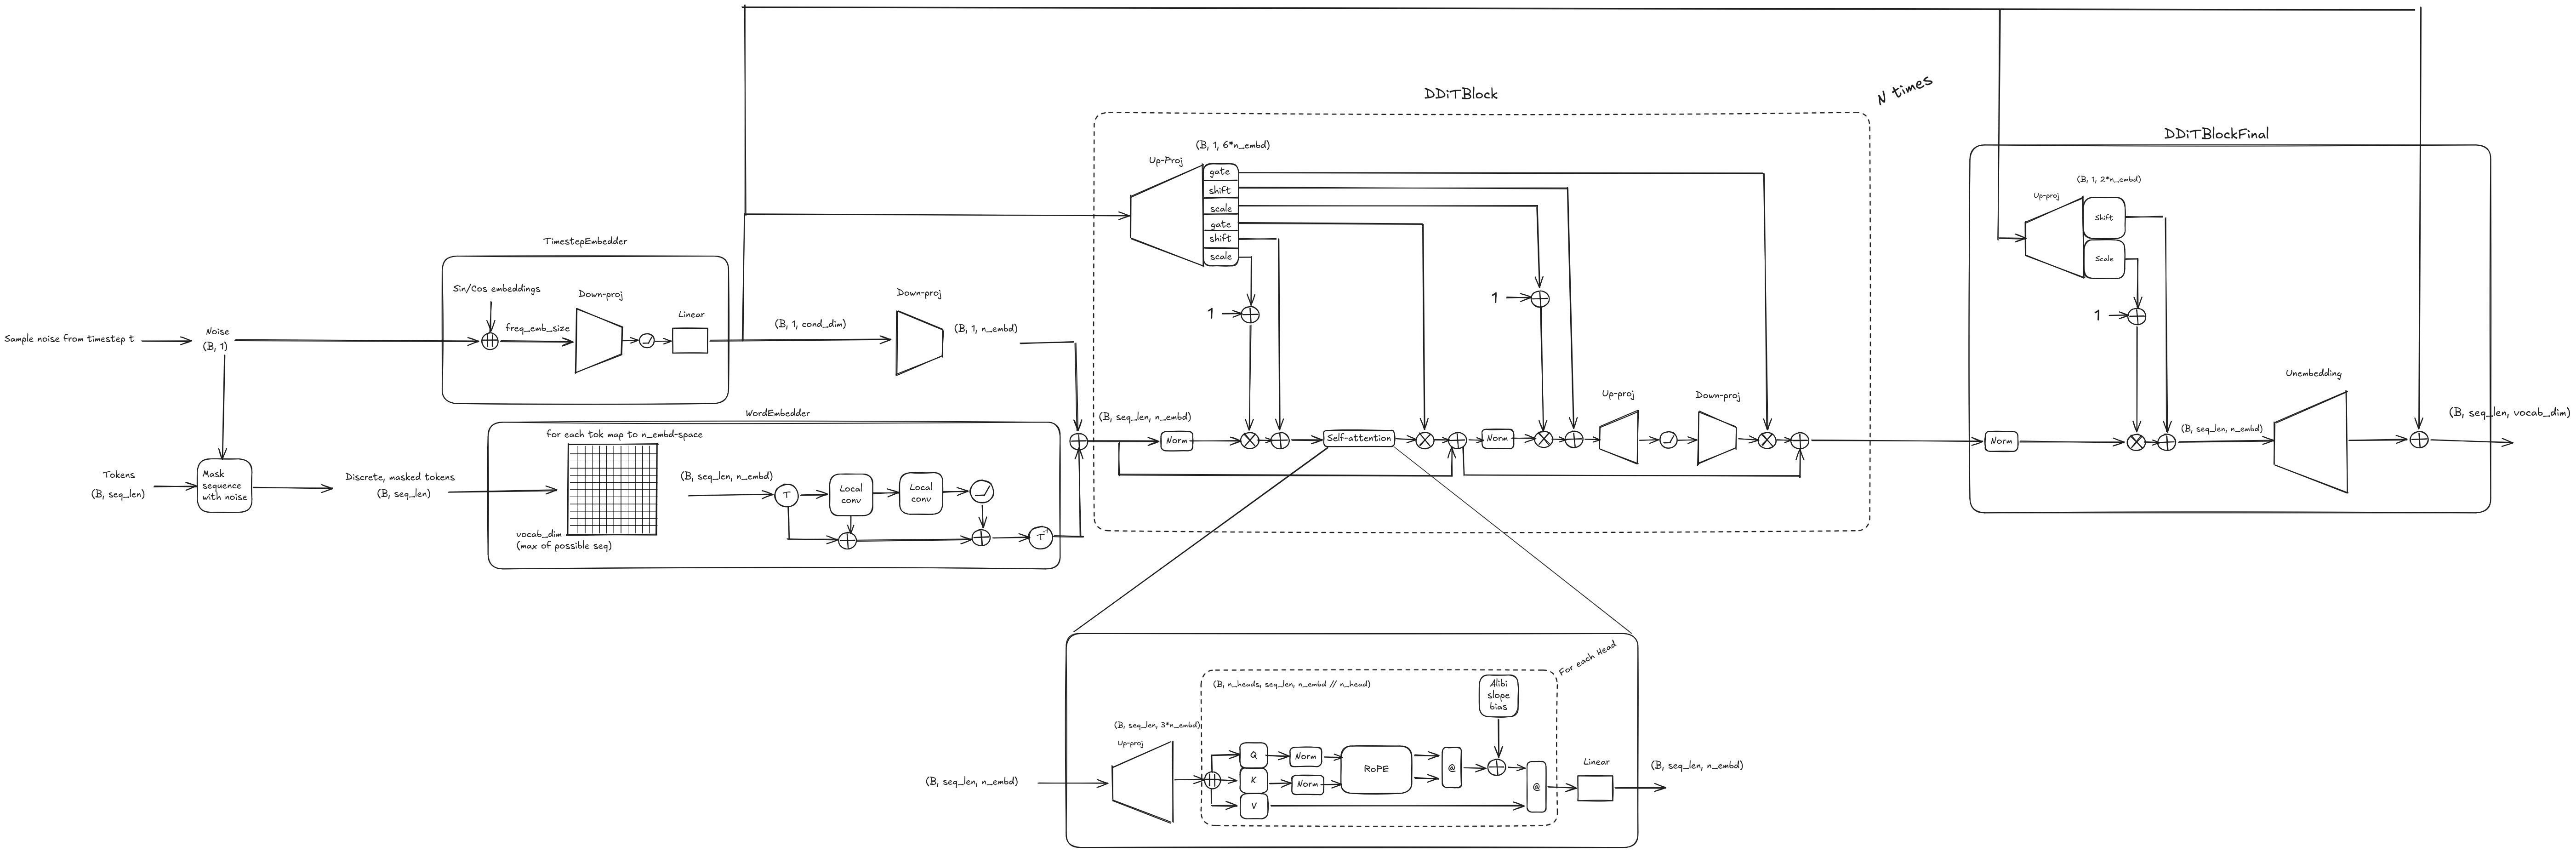
\includegraphics[width=0.92\linewidth]{full_arch.png}
  \caption{The diffusion transformer backbone. A scalar noise level $\sigma$ is
  embedded and used both for per-block adaLN modulation (shift, scale, gate) and
  for direct embedding-level and logit-level bypass projections. Token
  embeddings pass through a stack of depthwise convolutions (left, ``local
  conv'') before entering the transformer blocks (Section~\ref{sec:conv}).}
  \label{fig:arch}
\end{figure*}

\section{Convolutional Preprocessing of Token Embeddings}
\label{sec:conv}

A standard transformer block mixes information across positions only through
self-attention, so at the character level the model must learn even the most
local structure, such as common digraphs, morphemes, and word boundaries, from
attention alone. We instead give the model an explicit local operator by
convolving the token embeddings before they enter the transformer. After the
embedding lookup produces $h$, we apply a residual stack of two depthwise
(groups $=n_{\text{embd}}$) one-dimensional convolutions with kernel size 3 and a
nonlinearity before the second:
\begin{align}
  h &\leftarrow h + \mathrm{DWConv}_3(h), \label{eq:conv1}\\
  h &\leftarrow h + \mathrm{DWConv}_3\big(\mathrm{SiLU}(h)\big). \label{eq:conv2}
\end{align}
The two convolutions give an effective receptive field of five characters with a
nonlinear interaction between them, and both are residual, so the stack starts
near the identity and gradually specializes into local feature detectors. This
is the only convolutional component in the final model; it acts once, on the
embeddings, and not inside the transformer blocks.

The addition is inexpensive. A depthwise convolution with kernel size $k$ over an
embedding of width $n_{\text{embd}}$ has $n_{\text{embd}}\cdot k$ weights, so the
two layers add $2 \cdot 384 \cdot 3 = 2{,}304$ parameters, under $0.04\%$ of the
budget. Its forward cost is $\mathcal{O}(n_{\text{embd}} k\, T)$ for a length-$T$
sequence, negligible next to the $\mathcal{O}(T^2 n_{\text{embd}})$ attention and
$\mathcal{O}(T\, n_{\text{embd}}^2)$ feed-forward cost of even one block: the two
convolutions add about $4.6$ kFLOPs per token, $0.04\%$ of the
${\sim}12.4$ MFLOPs per token of the full three-layer forward pass.

\begin{table}[t]
  \centering
  \small
  \setlength{\tabcolsep}{4pt}
  \begin{tabular}{lccc}
    \toprule
    \textbf{Addition} & \textbf{Val.\ red.} & \textbf{Params} & \textbf{Compute} \\
    \midrule
    Embedding conv stack   & $0.9\%$ & $2{,}304$ & $+0.04\%$ \\
    Register tokens ($8$)  & $0.6\%$ & $3{,}072$ & $+2.4\%$ \\
    Context $384{\to}512$  & $0.5\%$ & $0$       & $+4.8\%$ \\
    \bottomrule
  \end{tabular}
  \caption{Validation-loss reduction (relative) versus cost for three additions
  in the cross-entropy ablation. Compute is the increase in forward-pass FLOPs
  per trained token over the $T{=}384$ baseline (${\sim}12.4$ MFLOPs/token).
  The embedding convolution gives the largest reduction of the three while
  adding few parameters and almost no compute; register tokens send $8$ extra
  positions through every layer and enlarge the quadratic attention term, and a
  longer context window grows per-token attention cost linearly in $T$
  (per-sequence cost quadratically).}
  \label{tab:cost}
\end{table}

In the controlled ablation, introducing the convolution on the embeddings
reduced validation loss by about $0.5\%$, and deepening it into the two-layer
stack of Equations~\ref{eq:conv1}--\ref{eq:conv2} reduced it by a further
$0.4\%$, for a combined reduction of roughly $0.9\%$. Table~\ref{tab:cost} places
this against two other changes of similar magnitude. The convolution achieves the
largest of the three reductions while adding fewer parameters than the register
tokens and far less compute than the longer context window, making it one of the
most cost-effective changes in the study.

The benefit was not only quantitative. Of all the changes we made, the embedding
convolution produced the clearest improvement in sample quality: the
pre-convolution model tended to emit degenerate repetitions such as
``your \ldots\ your \ldots\ your'', whereas the convolutional model produced
well-formed words, plausible character names, and sentence-like structure. This
is consistent with the mechanism, since a depthwise convolution is a direct
inductive bias for the short-range, position-local correlations (spelling and
common $n$-grams) that dominate character-level text and that parallel,
order-agnostic denoising otherwise has to recover through attention. The
receptive field mattered: kernel size 3 (receptive field 5 when stacked)
outperformed kernel size 5 and dilated variants, indicating that tight locality
is what helps. The recipe is also specific: normalizing before each convolution,
applying it before rather than after the residual embedding, zero-initializing
the convolutions, and adding a convolution on the final pre-logit representation
all regressed. Convolutions inside every transformer block helped under the
cross-entropy proxy but gave no reliable benefit under score-entropy, so the
final model keeps only the single embedding-level stack.

\section{Ablation Study}
\label{sec:ablation}

Each experiment tests one hypothesis under the same two-epoch benchmark; a change
is kept only if it lowers validation loss. This greedy procedure over about 105
experiments produced the cumulative milestones in Table~\ref{tab:milestones};
most candidate changes landed at or above the running best, showing how few
actually help in this regime.

\begin{table}[t]
  \centering
  \small
  \setlength{\tabcolsep}{4pt}
  \begin{tabular}{lcc}
    \toprule
    \textbf{Milestone} & \textbf{Val.\ loss} & \textbf{Cum.\ red.} \\
    \midrule
    Baseline (default config)          & 1.0268 & --- \\
    \;+ timestep ($\sigma$) embedding  & 1.0105 & $1.6\%$ \\
    \;+ RoPE                           & 0.9152 & $10.9\%$ \\
    \;+ embedding convolutions         & 0.8832 & $14.0\%$ \\
    \;+ ALiBi and QK-Norm              & 0.8770 & $14.6\%$ \\
    \;+ cosine LR with warm restarts   & 0.8531 & $16.9\%$ \\
    \;+ weight averaging (decay 0.998) & 0.8203 & $20.1\%$ \\
    \;+ batch-size tuning              & 0.7960 & $22.5\%$ \\
    Final                              & 0.7920 & $22.9\%$ \\
    \bottomrule
  \end{tabular}
  \caption{Cumulative milestones of the autonomous search on the cross-entropy
  ablation path, with reduction relative to the baseline. Note that the improvements are dependent/aggregate.}
  \label{tab:milestones}
\end{table}

Beyond the embedding convolution, the largest single improvement was RoPE
\citep{su2021rope}, which replaced learned positional embeddings and reduced
validation loss by about $4.4\%$, with smaller additional gains from the
learnable per-head ALiBi locality bias \citep{press2022alibi} and query-key
normalization \citep{henry2020qknorm}. Direct noise-level conditioning, obtained
by scaling the noise level before the sinusoidal embedding and adding
zero-initialized projections of it at the embedding and logit levels, gave
consistent small gains. On the optimization side, the Muon optimizer
\citep{jordan2024muon} applied to the two-dimensional weight matrices, with AdamW
for the rest, tolerated a learning rate roughly twice that of AdamW; a cosine
schedule with warm restarts \citep{loshchilov2017sgdr} at one cycle per epoch,
together with exponential moving averaging of the weights for evaluation,
contributed the largest optimization gains. Smaller batch sizes (around 96) also
outperformed larger ones, as more frequent updates and higher gradient noise
improved generalization within the fixed budget.

Many plausible modern techniques regressed. Mixture-of-experts
\citep{shazeer2017moe}, gated linear-attention layers, and SwiGLU feed-forwards
\citep{shazeer2020glu} all hurt: in a 3-layer, two-epoch model the gating and
routing mechanisms never get enough steps to specialize, and any reduction in
dense feed-forward capacity is not recovered. Sharpness-aware minimization
\citep{foret2021sam} doubled compute and still made validation worse; stochastic
weight averaging \citep{izmailov2018swa} underperformed the exponential moving
average, because the model is still improving monotonically, so any equal-weight
window over snapshots includes worse early ones; and span masking broke the
per-token independence assumed by the score-entropy derivation. 

A consistent lesson is that optimization choices are at least as important as architectural ones in this regime. In particular, exponential weight averaging gives one of the largest improvements on the cumulative search path. This does not invalidate the convolution result: weight averaging is an established, broadly applicable optimization technique, whereas the input convolution is a cheap task-specific architectural bias. The milestone path used masked cross-entropy; the convolution benefit was also observed under score-entropy.

\section{Generated Samples}
\label{sec:samples}

Figure~\ref{fig:sample} shows a sample from the final model (averaged weights,
256 unmasking steps) from a fully masked sequence. A model of this size and
budget does not produce semantically coherent passages, but the sample reproduces
salient features of the corpus: speaker labels in capitals followed by a colon
(\texttt{MENENIUS:}) appear in the correct position; the vocabulary and
morphology are largely well-formed (\texttt{your honour},
\texttt{crook'd upon my gage}); and the line lengths and punctuation follow the
dramatic-verse layout of the source. The errors are mostly local
(\texttt{thae} for \texttt{the}, \texttt{mame} for \texttt{name}), as expected
from a character-level model that has captured local orthographic and structural
regularities but not long-range meaning. This matches the quantitative picture,
since the embedding convolution improves exactly this kind of local structure and
was also the change that most visibly improved the samples.

\begin{figure}[t]
  \centering
  \footnotesize
\begin{verbatim}
 to take your honour to you, my lord.

MENENIUS:
I will not come to have them, for you
  have you need,
To give me with your honour to your
  consent,
And you are your honour and your mother,
Your honour save you yet thae more,
You have done to the matters of the
  cause;
But the time shall be crook'd upon my
  gage,
And make my hearted  the house of the
  nose,
That he is no more that mame
\end{verbatim}
  \caption{A sample from the final model. Speaker labels, archaic vocabulary, and
  verse layout are reproduced; the remaining errors are local. Long lines are
  wrapped to fit the column.}
  \label{fig:sample}
\end{figure}

\section{Forward-Pass Cost}
\label{sec:perf}

Because diffusion sampling repeats the forward pass once per denoising step,
forward-pass latency directly determines generation cost. We optimized the
forward pass of the 6.47M-parameter model at the kernel level. Compilation with
\texttt{torch.compile} gave a $1.58\times$ speedup, from 32.9~ms to 20.8~ms, and
replacing the hottest operations with custom Triton kernels
\citep{tillet2019triton} reached $1.81\times$, at 18.2~ms. Since unmasking uses
256 steps, these constant-factor gains compound directly into end-to-end
sampling throughput. This gives us a generation speed of around 110 tokens/s, 
which is comparable to frontier models such as Gemini 3.1 Pro Preview.

\section{Conclusion}

In this character-level discrete diffusion setting, the clearest architectural result was a small residual stack of depthwise convolutions on the token embeddings. The final input-only stack adds about 2,300 parameters and negligible computation, while improving validation loss and producing the clearest qualitative improvement in local text structure. Optimization mattered at least as much: exponential weight averaging produced a similarly strong gain along the search trajectory and would reasonably form part of a stronger baseline in future work. We therefore view the convolution not as the dominant source of overall improvement, but as evidence that an explicit and inexpensive local operator can complement global attention in small character-level diffusion models.

\section*{Limitations}

The study is confined to one small dataset (Tiny Shakespeare) at the character
level, one model under 6.5M parameters, a fixed two-epoch budget, and largely a
single seed, so absolute numbers and the sign of some effects may differ at
scale, on subword tokenization, or with longer training. The autonomous search
is a greedy hill-climb that commits on small validation-loss differences, some
within run-to-run noise, so the path is not guaranteed optimal. Finally,
validation loss is an imperfect proxy for generation quality, and the qualitative
claims rest on sample inspection rather than human evaluation.

\section*{Acknowledgments}

This project was part of a Claude Code evaluation. AI assistance was used for the
autonomous ablation loop, plotting, and debugging; all hypotheses and final
configurations were verified by the author.

\bibliography{custom}

\end{document}
